\documentclass[12pt,preprint, authoryear]{elsarticle}

\usepackage{lmodern}
%%%% My spacing
\usepackage{setspace}
\setstretch{1.5}
\DeclareMathSizes{12}{14}{10}{10}

% Wrap around which gives all figures included the [H] command, or places it "here". This can be tedious to code in Rmarkdown.
\usepackage{float}
\let\origfigure\figure
\let\endorigfigure\endfigure
\renewenvironment{figure}[1][2] {
    \expandafter\origfigure\expandafter[H]
} {
    \endorigfigure
}

\let\origtable\table
\let\endorigtable\endtable
\renewenvironment{table}[1][2] {
    \expandafter\origtable\expandafter[H]
} {
    \endorigtable
}


\usepackage{ifxetex,ifluatex}
\usepackage{fixltx2e} % provides \textsubscript
\ifnum 0\ifxetex 1\fi\ifluatex 1\fi=0 % if pdftex
  \usepackage[T1]{fontenc}
  \usepackage[utf8]{inputenc}
\else % if luatex or xelatex
  \ifxetex
    \usepackage{mathspec}
    \usepackage{xltxtra,xunicode}
  \else
    \usepackage{fontspec}
  \fi
  \defaultfontfeatures{Mapping=tex-text,Scale=MatchLowercase}
  \newcommand{\euro}{€}
\fi

\usepackage{amssymb, amsmath, amsthm, amsfonts}

\def\bibsection{\section*{References}} %%% Make "References" appear before bibliography


\usepackage[round]{natbib}

\usepackage{longtable}
\usepackage[margin=2.3cm,bottom=2cm,top=2.5cm, includefoot]{geometry}
\usepackage{fancyhdr}
\usepackage[bottom, hang, flushmargin]{footmisc}
\usepackage{graphicx}
\numberwithin{equation}{section}
\numberwithin{figure}{section}
\numberwithin{table}{section}
\setlength{\parindent}{0cm}
\setlength{\parskip}{1.3ex plus 0.5ex minus 0.3ex}
\usepackage{textcomp}
\renewcommand{\headrulewidth}{0.2pt}
\renewcommand{\footrulewidth}{0.3pt}

\usepackage{array}
\newcolumntype{x}[1]{>{\centering\arraybackslash\hspace{0pt}}p{#1}}

%%%%  Remove the "preprint submitted to" part. Don't worry about this either, it just looks better without it:
\makeatletter
\def\ps@pprintTitle{%
  \let\@oddhead\@empty
  \let\@evenhead\@empty
  \let\@oddfoot\@empty
  \let\@evenfoot\@oddfoot
}
\makeatother

 \def\tightlist{} % This allows for subbullets!

\usepackage{hyperref}
\hypersetup{breaklinks=true,
            bookmarks=true,
            colorlinks=true,
            citecolor=blue,
            urlcolor=blue,
            linkcolor=blue,
            pdfborder={0 0 0}}


% The following packages allow huxtable to work:
\usepackage{siunitx}
\usepackage{multirow}
\usepackage{hhline}
\usepackage{calc}
\usepackage{tabularx}
\usepackage{booktabs}
\usepackage{caption}


\newenvironment{columns}[1][]{}{}

\newenvironment{column}[1]{\begin{minipage}{#1}\ignorespaces}{%
\end{minipage}
\ifhmode\unskip\fi
\aftergroup\useignorespacesandallpars}

\def\useignorespacesandallpars#1\ignorespaces\fi{%
#1\fi\ignorespacesandallpars}

\makeatletter
\def\ignorespacesandallpars{%
  \@ifnextchar\par
    {\expandafter\ignorespacesandallpars\@gobble}%
    {}%
}
\makeatother

\newlength{\cslhangindent}
\setlength{\cslhangindent}{1.5em}
\newenvironment{CSLReferences}%
  {\setlength{\parindent}{0pt}%
  \everypar{\setlength{\hangindent}{\cslhangindent}}\ignorespaces}%
  {\par}


\urlstyle{same}  % don't use monospace font for urls
\setlength{\parindent}{0pt}
\setlength{\parskip}{6pt plus 2pt minus 1pt}
\setlength{\emergencystretch}{3em}  % prevent overfull lines
\setcounter{secnumdepth}{5}

%%% Use protect on footnotes to avoid problems with footnotes in titles
\let\rmarkdownfootnote\footnote%
\def\footnote{\protect\rmarkdownfootnote}
\IfFileExists{upquote.sty}{\usepackage{upquote}}{}

%%% Include extra packages specified by user

%%% Hard setting column skips for reports - this ensures greater consistency and control over the length settings in the document.
%% page layout
%% paragraphs
\setlength{\baselineskip}{12pt plus 0pt minus 0pt}
\setlength{\parskip}{12pt plus 0pt minus 0pt}
\setlength{\parindent}{0pt plus 0pt minus 0pt}
%% floats
\setlength{\floatsep}{12pt plus 0 pt minus 0pt}
\setlength{\textfloatsep}{20pt plus 0pt minus 0pt}
\setlength{\intextsep}{14pt plus 0pt minus 0pt}
\setlength{\dbltextfloatsep}{20pt plus 0pt minus 0pt}
\setlength{\dblfloatsep}{14pt plus 0pt minus 0pt}
%% maths
\setlength{\abovedisplayskip}{12pt plus 0pt minus 0pt}
\setlength{\belowdisplayskip}{12pt plus 0pt minus 0pt}
%% lists
\setlength{\topsep}{10pt plus 0pt minus 0pt}
\setlength{\partopsep}{3pt plus 0pt minus 0pt}
\setlength{\itemsep}{5pt plus 0pt minus 0pt}
\setlength{\labelsep}{8mm plus 0mm minus 0mm}
\setlength{\parsep}{\the\parskip}
\setlength{\listparindent}{\the\parindent}
%% verbatim
\setlength{\fboxsep}{5pt plus 0pt minus 0pt}



\begin{document}



\begin{frontmatter}  %

\title{Question 4}

% Set to FALSE if wanting to remove title (for submission)




\author[Add1]{Sahil Bhugwan}
\ead{21075492@sun.ac.za}





\address[Add1]{Github- \url{https://github.com/SBhugwan}}


\begin{abstract}
\small{
Given the age of streaming launching a new streaming serives is the way
to go however questions must be asked given Netflix recent decline. This
will look to see if SU Streaming should lauch its own service.
}
\end{abstract}

\vspace{1cm}


\begin{keyword}
\footnotesize{
Netflix \textbackslash{} \\
\vspace{0.3cm}
}
\end{keyword}



\vspace{0.5cm}

\end{frontmatter}



%________________________
% Header and Footers
%%%%%%%%%%%%%%%%%%%%%%%%%%%%%%%%%
\pagestyle{fancy}
\chead{}
\rhead{}
\lfoot{}
\rfoot{\footnotesize Page \thepage}
\lhead{}
%\rfoot{\footnotesize Page \thepage } % "e.g. Page 2"
\cfoot{}

%\setlength\headheight{30pt}
%%%%%%%%%%%%%%%%%%%%%%%%%%%%%%%%%
%________________________

\headsep 35pt % So that header does not go over title




\hypertarget{introduction}{%
\section{\texorpdfstring{Introduction
\label{Introduction}}{Introduction }}\label{introduction}}

There are multiple streaming services in the world such as Disney plus,
Netflix etc. However Netflix was one of the first streaming services in
the world. However the question remains has the market become to
saturated given the decline in Netflix users

\hypertarget{trends-over-time}{%
\section{Trends Over time}\label{trends-over-time}}

The first thing that i will be looking at is the content on Netflix over
time

\begin{figure}[H]

{\centering \includegraphics{Q4_files/figure-latex/Figure1-1} 

}

\caption{Content on Netflix over time \label{Figure1}}\label{fig:Figure1}
\end{figure}

It can be see from this graph that from the late 1990s netflix really
starting to take off. However from 2010 there was an explosion in the
content. this lasted up an till 2015 as other streaming services started
to enter the market.

\hypertarget{distribution-of-content}{%
\section{Distribution of Content}\label{distribution-of-content}}

Given that Netflix is a streaming platform it offers both movies and
shows

\begin{figure}[H]

{\centering \includegraphics{Q4_files/figure-latex/Figure2-1} 

}

\caption{Pie chart of content \label{Figure2}}\label{fig:Figure2}
\end{figure}

Is is clearly evident from figure \ref{Figure2} that Netflix offers more
movies than shows. To look as this more clearly we will look the bar
chart to show the difference in content

\begin{figure}[H]

{\centering 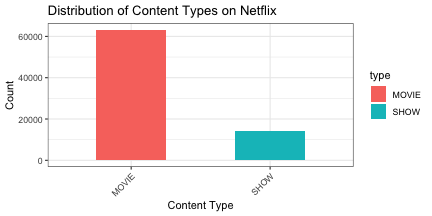
\includegraphics{Q4_files/figure-latex/Figure3-1} 

}

\caption{Bar graph \label{Figure3}}\label{fig:Figure3}
\end{figure}

It is clearly evident that netflix platform hosts more movies that
shows.

However one must question whether given that shows dominate on netflix
how do they rate compared to shows.

\begin{figure}[H]

{\centering \includegraphics{Q4_files/figure-latex/Figure4-1} 

}

\caption{Average ratings  \label{Figure4}}\label{fig:Figure4}
\end{figure}

\begin{verbatim}
##    age_certification num_titles
## 1                  G       1456
## 2              NC-17        258
## 3                 PG       5134
## 4              PG-13      11508
## 5                  R      15853
## 6              TV-14       3518
## 7               TV-G        377
## 8              TV-MA       6581
## 9              TV-PG        944
## 10              TV-Y        299
## 11             TV-Y7        667
\end{verbatim}

\hypertarget{popular-people-on-netflix}{%
\section{Popular people on Netflix~}\label{popular-people-on-netflix}}

If SU wants to launch its own service it should consider which
actors/actress has the most content on netflix

\begin{figure}[H]

{\centering \includegraphics{Q4_files/figure-latex/Figure6-1} 

}

\caption{Common Stars on Netflix  \label{Figure1}}\label{fig:Figure6}
\end{figure}

Therefore Shah Rukh Khan has the most content on netflix, thus if SU has
its own streaming service it should include some of his content. This is
because if we look at the Figure 4.2 we can see that he has a high
popularity as well as the content he is in tends to be rated above 6 on
IMDb.

\begin{figure}[H]

{\centering \includegraphics{Q4_files/figure-latex/Figure7-1} 

}

\caption{Correlation \label{Figure3}}\label{fig:Figure7}
\end{figure}

\hypertarget{content-by-country}{%
\section{Content By Country}\label{content-by-country}}

Given that SU will be launching a streaming service in South Africa
first and then branch out into the world. Given this it can be seen
below that America produces the most content on netflix.

\begin{figure}[H]

{\centering \includegraphics{Q4_files/figure-latex/Figure8-1} 

}

\caption{Content Produced by Country \label{Figure1}}\label{fig:Figure8}
\end{figure}

Therefore for SU to be unique it should potential look to produce it own
unique content.

What SU could possible do is look as genres that have the most dominate
genres

\begin{figure}[H]

{\centering \includegraphics{Q4_files/figure-latex/Figure9-1} 

}

\caption{Word cloud most dominate genres \label{Figure2}}\label{fig:Figure9}
\end{figure}

Therefore it can bee see that drama and comedy are the most popular
content on netflix

\hypertarget{conclusion}{%
\section{Conclusion}\label{conclusion}}

Therefore if SU launches it sown streaming service it must ensure that
it has a lot of movies for it users. It should also have high content of
Drama. Thus a possibility if for them to produce there own content with
one of the top actors/actress these will help ensure that it is
successful.

\bibliography{Tex/ref}





\end{document}
